%% ─────────────────────────────────────────────────────────────────────────
\subsection{Internal Research Context}
%% ─────────────────────────────────────────────────────────────────────────

\subsubsection{Smart Green Supply Chain Programme}


The \gls{din} of ALTEN conducts applied R\&D at the
intersection of digital twin technology, logistics optimisation, and sustainable
transport. 

The Smart Green Supply Chain programme~\autocite{benzakour2024history}
articulates three complementary pillars:

\begin{itemize}
    \item \textbf{Lean}: Minimisation of waste (cost, delay, over-stock) through
          pull-flow logic and real-time scheduling.
    \item \textbf{Green}: Minimisation of carbon footprint per transport leg, aligned with the \gls{glec} Framework v3.2~\autocite{smartfreight2023glec} and ISO~14083:2023~\autocite{iso14083}.
    \item \textbf{Predictive}: Anticipation of disruptions through probabilistic modelling and machine learning, consistent with the digital supply chain twin approach~\autocite{ivanov2020digital}.
\end{itemize}

This programme places ALTEN-DIN within the broader Industry~4.0 movement \autocite{kagermann2013industry}, which uses cyber-physical systems, \gls{iot}, and
digital twins to transform reactive supply chains into adaptive, self-organising networks.

The Physical Internet framework~\autocite{montreuil2011toward}, proposing
open, mutualized logistics networks analogous to internet routing protocols, provides the theoretical backdrop for the supply chain simulation environment described below.

\subsubsection{Project: DISCO Digital Twin}

DISCO (Supply Chain Illustrator) is a serious game and digital twin developed by the DIN to simulate a complete supply chain for a fictitious satellite product. It involves
22 component suppliers in domains such as structural assemblies, optical systems, and embedded electronics~\autocite{baxas2025architecture}. Players assume the role of
supply chain buyers and make decisions about supplier selection, transport routes, and factory allocation. The DISCO technology stack is summarised in Table~\ref{tab:disco_stack}.

\begin{figure}[H]
    \centering
    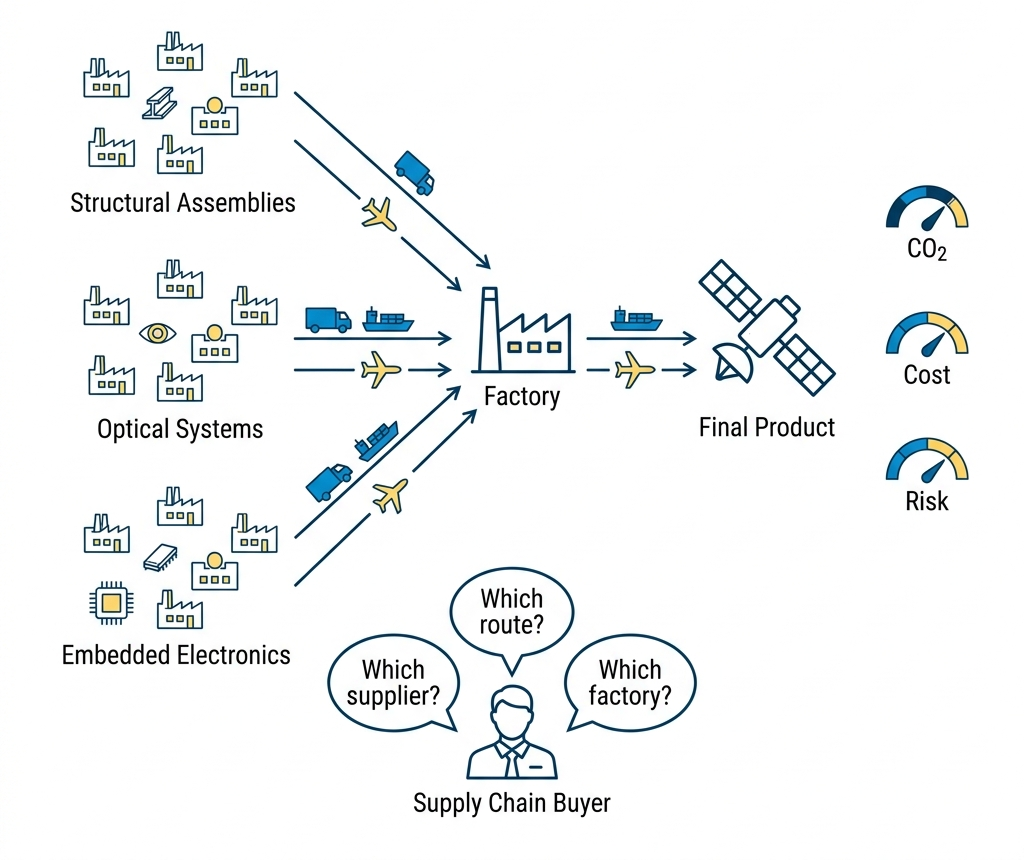
\includegraphics[width=0.85\linewidth]{Images/1.Introduction/disco_map.png}
    \caption{The DISCO serious game: 22 suppliers, transport decisions, and the three scored dimensions.}
    \label{fig:todraw_disco}
\end{figure}

The scoring engine applies Min-Max normalisation over the values of the current game
session:

	\begin{equation}
	    \text{ScoreCO}_2 = 1 + 9 \times \frac{\text{realCO}_2 - \text{co}_{2,\min}}
	                                         {\text{co}_{2,\max} - \text{co}_{2,\min}},
	    \label{eq:score_co2}
	\end{equation}
	
	The operational variables of the CO\textsubscript{2} scoring model are described in Table~\ref{tab:co2_components}.
	
	\begin{table}[H]
	\centering
	\caption{Component definitions for the CO\textsubscript{2} scoring equation.}
	\label{tab:co2_components}
	\small
	\begin{tabularx}{\linewidth}{llX}
	\toprule
	\textbf{Component} & \textbf{Type} & \textbf{Description} \\
	\midrule
	$\text{ScoreCO}_2$ & Dependent variable & Normalized greenhouse gas score on a $[1, 10]$ scale \\
	$\text{realCO}_2$  & Input variable     & Measured carbon emissions on the transport leg \\
	$\text{co}_{2,\min}$ & System parameter  & Minimum historical or target emissions threshold \\
	$\text{co}_{2,\max}$ & System parameter  & Maximum historical or target emissions threshold \\
	\bottomrule
	\end{tabularx}
	\end{table}

with analogous formulae for cost and risk. The scale ranges from 1 to 10, where 1 corresponds to the best possible performance and 10 to the worst.

To support the demonstration and continuous improvement of mature supply chain capabilities, the DISCO digital twin incorporates several specialized modules developed in prior research cycles: The routing module~\autocite{baulain2024internet}, the risk scorer~\autocite{kabouche2025scoring}, the CO\textsubscript{2} quantification methodology~\autocite{cordova2024green}, and the software integration framework~\autocite{auclin2025bst}.


	\begin{table}[ht]
	\centering
	\caption{DISCO technology stack and key parameters.}
	\label{tab:disco_stack}
	\begin{tabularx}{\linewidth}{lX}
	\toprule
	\textbf{Component} & \textbf{Technology / Value} \\
	\midrule
	Backend API    & Spring Boot + Java~21 \\
	Database       & PostgreSQL (Azure) \\
	Frontend       & Angular (localhost:4200) \\
	REST API (test) & \texttt{https://test-disco.altenlabs.net/back/} \\
	Authentication & Player key / Azure AD SSO OAuth2 \\
	Scores computed & CO\textsubscript{2}, Cost, Risk per supplier/itinerary [1–10] \\
	\bottomrule
	\end{tabularx}
	\end{table}

%% ─────────────────────────────────────────────────────────────────────────
\subsubsection{Capitalisation of Prior ALTEN-DIN Research}
%% ─────────────────────────────────────────────────────────────────────────

This R\&D operation is situated within a body of prior DIN research conducted under
the Smart Green Digital Supply Chain programme. These works form the organisational and thematic context of the present
operation; the system delivered here (SupplyScore, Section~\ref{sec:Operations}) is
a standalone Python application and does not integrate with these modules yet.
Their coupling is a stated perspective of the programme, not a
delivered capability.

\textbf{Baxas~\autocite{baxas2025architecture}} defines the DISCO software
architecture, including the \gls{tts}/\gls{ttr} formalisation.

\textbf{Baulain and Dubarry~\autocite{baulain2024internet}} developed the Physical
Internet routing module of DISCO, providing transit times via the HERE Maps API
(Vincenty distances, mandatory 4h30 \gls{hgv} pause compliance) and the Itinerary
Performance Index (\gls{ipg}) normalised in $[0,1]$.

\textbf{Kabouche~\autocite{kabouche2025scoring}} developed the supplier risk scorer
combining delay history, geographic vulnerability, and financial fragility into a
$[1, 10]$ scale.

\textbf{Cordova~\autocite{cordova2024green}} developed the CO\textsubscript{2}
quantification module per route using the GLEC/VECTO methodology with log-normalised
output $\hat{x}_{\text{CO}_2}$.

\textbf{Mondelice~\autocite{mondelice2025tms}} developed the Transport Management
System interface providing real-time transit-time extraction.


%% ─────────────────────────────────────────────────────────────────────────
\subsection{Document Structure}
%% ─────────────────────────────────────────────────────────────────────────

This document is structured as follows. Section~\ref{sec:Problem} formalises the scientific problem, states the operation's objectives, research questions and hypotheses, and outlines the primary research challenges. Section~\ref{sec:SOTA} reviews the state of the art across thematic subsections. Section~\ref{sec:Operations} details the R\&D iterations, the methodology, and the serious-game validation campaign. Finally, Section~\ref{sec:Conclusions} states the documented limitations of the delivered framework and closes with a personal assessment.
